\documentclass{beamer}
%
% Choose how your presentation looks.
%
% For more themes, color themes and font themes, see:
% http://deic.uab.es/~iblanes/beamer_gallery/index_by_theme.html
%
\mode<presentation>
{
  \usetheme{default}      % or try Darmstadt, Madrid, Warsaw, ...
  \usecolortheme{default} % or try albatross, beaver, crane, ...
  \usefonttheme{default}  % or try serif, structurebold, ...
  \setbeamertemplate{navigation symbols}{}
  \setbeamertemplate{caption}[numbered]
} 

\usepackage[english]{babel}
\usepackage[utf8]{inputenc}
\usepackage{bm}
\usepackage{biblatex}
\usepackage{bibentry}
\title{Probabilistic PCA and Extensions}
\author[Montemurri and Mhedhbi]
{Michael Montemurri\inst{1} \and Ahmed Mhedhbi\inst{2}}

\institute[Short Institute Name]{
    \inst{1} McGill University \\
    \inst{2} Université de Montréal
}
\date{December 2024}

\begin{document}

% Slide 1: Title Slide
\begin{frame}
    \titlepage
\end{frame}

\begin{frame}
    \frametitle{Fundamental Results of PPCA}
    \framesubtitle{\footnotesize Based on [Bishop and Tipping, 1999]}
\textbf{Goal of PPCA:}
To model high-dimensional data \( \mathbf{x}_n \in \mathbb{R}^d \) using a lower-dimensional latent representation \( \mathbf{z}_n \in \mathbb{R}^q \) with \( q < d \), while accounting for Gaussian noise \( \boldsymbol{\epsilon} \).

\vspace{1em}
\textbf{Generative Model:}
\[
    \mathbf{x}_n = \mathbf{W}\mathbf{z}_n + \boldsymbol{\mu} + \boldsymbol{\epsilon}_n, \quad \boldsymbol{\epsilon}_n \sim \mathcal{N}(0, \sigma^2 \mathbf{I}),
\]

 Where: \( \mathbf{W} \in \mathbb{R}^{d \times q} \): matrix mapping latent space to data space.

% \textbf{Complete Log-Likelihood:}
% \[
%     L(\mathbf{W}, \boldsymbol{\mu}, \sigma^2) = -\frac{N}{2}\left[d\ln(2\pi) + \ln |\mathbf{C}| + \operatorname{Tr}(\mathbf{C}^{-1}\mathbf{S})\right],
% \]
% where \( \mathbf{C} = \mathbf{W}\mathbf{W}^T + \sigma^2\mathbf{I} \) and \( \mathbf{S} \) is the sample covariance matrix.

\vspace{1em}

\textbf{Maximum Likelihood Estimation:}
\[
    \mathbf{W}_{\text{ML}} = \mathbf{U}_q(\boldsymbol{\Lambda}_q - \sigma^2\mathbf{I})^{1/2}\mathbf{R}, \quad \sigma^2_{\text{ML}} = \frac{1}{d - q} \sum_{j=q+1}^d \lambda_j,
\]
% where:
% \begin{itemize}
%     \item \( \mathbf{U}_q \): Top \( q \) eigenvectors of \( \mathbf{S} \).
%     \item \( \boldsymbol{\Lambda}_q \): Corresponding eigenvalues.
%     \item \( \lambda_{q+1}, \dots, \lambda_d \): Remaining eigenvalues.
% \end{itemize}

The generative framework allows us to apply the EM Algorithm to find $\mathbf{W}$ and $\sigma^2$, which can be computationally efficient for large $d$

\end{frame}

% \begin{frame}{The EM Algorithm for PPCA}

% \textbf{E-Step:}
% \[
% \mathbb{E}[\mathbf{z}_n | \mathbf{x}_n] = \mathbf{M}^{-1} \mathbf{W}^T (\mathbf{x}_n - \boldsymbol{\mu}),
% \]
% \[
% \mathbb{E}[\mathbf{z}_n \mathbf{z}_n^T | \mathbf{x}_n] = \sigma^2 \mathbf{M}^{-1} + \mathbb{E}[\mathbf{z}_n | \mathbf{x}_n]\mathbb{E}[\mathbf{z}_n | \mathbf{x}_n]^T,
% \]
% where \( \mathbf{M} = \mathbf{W}^T \mathbf{W} + \sigma^2 \mathbf{I} \).

% \vspace{1em}
% \textbf{M-Step:}
% \[
% \mathbf{W}_{\text{new}} = \mathbf{S} \mathbf{W} (\sigma^2 \mathbf{I} + \mathbf{M}^{-1} \mathbf{W}^T \mathbf{S} \mathbf{W})^{-1},
% \]
% \[
% \sigma^2_{\text{new}} = \frac{1}{d} \left[ \operatorname{Tr}(\mathbf{S}) - \operatorname{Tr}(\mathbf{S} \mathbf{W}\mathbf{M}^{-1}\mathbf{W}_{\text{new}}^T) \right].
% \]

% \vspace{1em}
% \textbf{Dimensions and Notation:}
% \begin{itemize}
%     \item \( \mathbf{z}_n \in \mathbb{R}^q \): Latent variables.
%     \item \( \mathbf{x}_n \in \mathbb{R}^d \): Observed data.
%     \item \( \mathbf{S} \in \mathbb{R}^{d \times d} \): Sample covariance matrix.
% \end{itemize}
% \end{frame}

% Slide 4: Mixture of PPCA Models, Bishop and Tipping
\begin{frame}
    \frametitle{Mixture of PPCA Models}
    \framesubtitle{\footnotesize Based on [Tipping and Bishop, 1999]}

    Generative Model:
    \[
     p(x_n) = \sum_{k=1}^K \pi_k \mathcal{N}(x_n|\mu_k, C_k) \quad C_k = W_kW_k^T + \sigma_k^2I
    \]
    
    Introduction of Posterior responsibilities:
    \[
     r_{nk} = p(z_n = k | \mathbf{x}_n) = \frac{\pi_k \mathcal{N}(\mathbf{x}_n | \boldsymbol{\mu}_k, \mathbf{C}_k)}{\sum_{j=1}^K \pi_j \mathcal{N}(\mathbf{x}_n | \boldsymbol{\mu}_j, \mathbf{C}_j)}.
    \]
    
    Use the EM algorithm to update all parameters simultaneously.
    
    % Include small diagram of mixture model in the bottom right
    \begin{figure}[b]
        \centering
        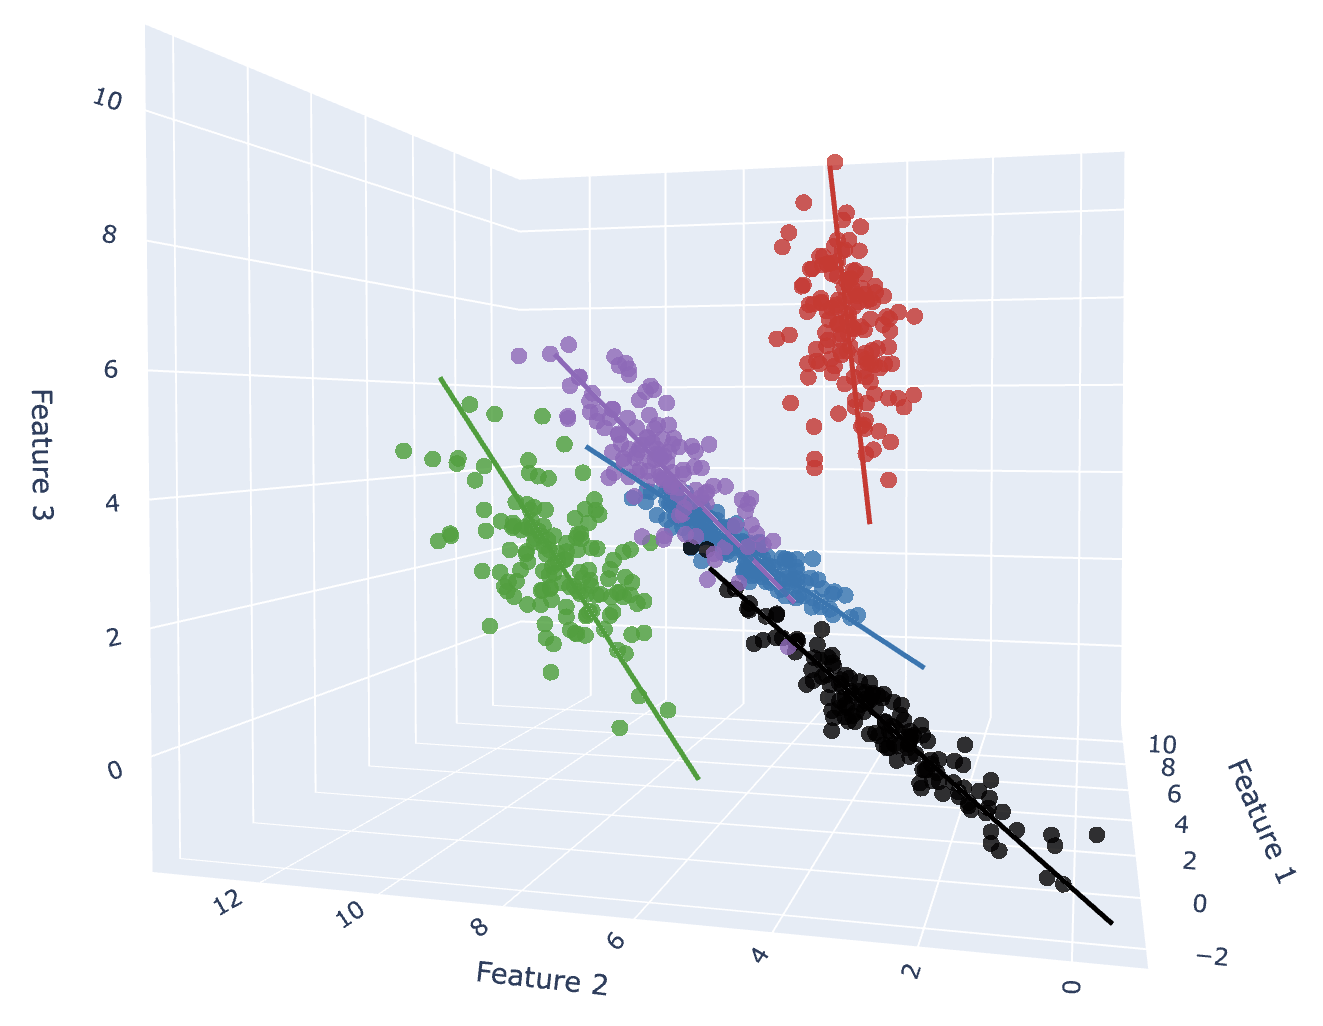
\includegraphics[width=0.4\textwidth]{3dcluster.png} % Replace with your diagram.
        \caption{Mixture of PPCA Models}
    \end{figure}
    
    \end{frame}

% Slide 5 PKPCA Zhang et al.
\begin{frame}
    \frametitle{Probabilistic Kernel PCA (PKPCA)}
    \framesubtitle{\footnotesize Based on [Zhang et al., 1999]}

        %\textbf{Theorem:} Let \( r < \infty \) and \( g_1, g_2, \dots, g_r \) be independent random vectors normally distributed as \( N(0, \Sigma) \). Then the kernel matrix \( K \sim W_n(r, \Sigma) \) when \( r \geq n \) and \( K \sim SW_n(r, \Sigma) \) when \( r < n \). Conversely, if \( K \sim W_n(r, \Sigma) \) or \( K \sim SW_n(r, \Sigma) \), there exist \( r \) mutually independent vectors \( \{g_j\}_{j=1}^r \) following \( N(0, \Sigma) \).
        
        % \vspace{1em}
        % \textbf{Motivation:}
        % \begin{itemize}
        %     \item PCA is limited to linear transformations.
        %     \item Kernel PCA (KPCA) uses the kernel trick to extend PCA to nonlinear transformations.
        %     \item Probabilistic Kernel PCA (PKPCA) extends PPCA to kernel-induced feature spaces using the same kernel trick.
        % \end{itemize}
        
        \vspace{1em}
        \textbf{Generative Model:} In the feature space \( \mathcal{F} \), we assume:
        \[
            \mathbf{g} = \mathbf{B} \mathbf{w} + u \mathbf{1}_n + \boldsymbol{\epsilon}, \quad \boldsymbol{\epsilon} \sim \mathcal{N}(0, \mathbf{V}),
        \]
        where:
        \begin{itemize}
            \item \( \mathbf{g} \in \mathbb{R}^n \): feature vector in the kernel-induced space.
            \item \( \mathbf{B} \in \mathbb{R}^{n \times m} \): weight matrix mapping latent variables \( \mathbf{w} \in \mathbb{R}^m \) to the feature space.
            \item \( u \mathbf{1}_n \): scalar bias term for mean.
            \item \( \boldsymbol{\epsilon} \sim \mathcal{N}(0, \mathbf{V}) \): noise term.
        \end{itemize}

        $ \bf{V} = n\sigma^2\bf{I}_n/r $ and $ w \sim \mathcal{N}(0, n\bf{I}_m/r) $.
        but r, the dimensionality of the feature space, is unknown. We use the kernel trick to yield estimation procedure for $\mathbf{B}$ and $\sigma^2$.
        \vspace{1em}
        \textbf{Main Result:} The kernel matrix \( K \) is a Wishart random matrix \( W_n(r, \Sigma) \), allowing a probabilistic generative model in the kernel space. This provides probabilistic interpretation of KPCA.
        \vspace{1em}
        
        \end{frame}

%Slide 7
% \begin{frame}{EM Algorithm for Matrix-Variate PKPCA}
%             \textbf{E-Step:} Compute the expectations:
%             \[
%             \begin{aligned}
%                 \mathbb{E}[W | F] &= D^{-1}B^\top(F - \mathbf{1}_n \mathbf{u}^\top), \\
%                 \mathbb{E}[WW^\top | F] &= n\sigma^2 D^{-1} + D^{-1} B^\top HKH B D^{-1},
%             \end{aligned}
%             \]
%             where \( D = B^\top B + \sigma^2 I_m \) and \( H = I_n - \frac{1}{n}\mathbf{1}_n \mathbf{1}_n^\top \).
            
%             \textbf{M-Step:} Update parameters \( B \) and \( \sigma^2 \):
%             \[
%             \begin{aligned}
%                 B^{(t+1)} &= (F - \mathbf{1}_n \mathbf{u}^\top) \mathbb{E}[W^\top | F] \big( \mathbb{E}[WW^\top | F] \big)^{-1}, \\
%                 \sigma^2_{(t+1)} &= \frac{1}{n^2} \Big( \text{tr}(HKH) + \text{tr}\big(\mathbb{E}[WW^\top | F] B^\top_{(t+1)} B_{(t+1)}\big) \\
%                 &\quad - 2 \text{tr}\big(B_{(t+1)} \mathbb{E}[W | F]^\top (F - \mathbf{1}_n \mathbf{u}^\top)^\top \big) \Big).
%             \end{aligned}
%             \]
            
%             \textbf{Initialization:}
%             \begin{itemize}
%                 \item Initialize \( B \) using the principal eigenvectors of \( H K H \).
%                 \item Initialize \( \sigma^2 \) based on the eigenvalues of \( H K H \).
%             \end{itemize}
            
%             \textbf{Repeat:}
%             \begin{itemize}
%                 \item Alternate between the E-step and M-step until convergence.
%             \end{itemize}
% \end{frame}

\begin{frame}{Summary of PKPCA and Comparison to PPCA}

    \textbf{Goal:}
    Extend probabilistic PCA (PPCA) to nonlinear relationships by leveraging the kernel trick to model data in a high-dimensional feature space \( \mathcal{F} \).
    
    \vspace{1em}
    \textbf{Generative Model in \( \mathcal{F} \):}
    \[
        \mathbf{g} = \mathbf{B} \mathbf{w} + u \mathbf{1}_n + \boldsymbol{\epsilon}, \quad \boldsymbol{\epsilon} \sim \mathcal{N}(0, \mathbf{V}),
    \]
    where \( \mathbf{g} \) is the feature vector, \( \mathbf{B} \) maps latent variables \( \mathbf{w} \) to \( \mathcal{F} \), and \( \mathbf{K} \sim W_n(r, \Sigma) \) is a Wishart random matrix.
    
    \vspace{1em}

    \begin{itemize}
            \item Models feature vectors \( \mathbf{g} \) in the kernel-induced feature space \( \mathcal{F} \).
            \item Uses the kernel trick to enable nonlinear dimensionality reduction.
            \item Probabilistic interpretation of the kernel matrix \( \mathbf{K} \) as a Wishart random matrix.
    \end{itemize}
    

    \end{frame}

%SLide 8
\begin{frame}{Original Contributions}

\end{frame}

% Slide 9: Experimental Results
\begin{frame}{Experimental Results}
\textbf{Comparison of Analytical and EM-Based PPCA:}
\textbf{Mixture Models:}

Mixture of PPCA models demonstrated superior performance in clustering multimodal datasets, capturing local linear structures effectively.

\textbf{PKPCA:}

Probabilistic Kernel PCA significantly outperformed linear PPCA in modeling complex, nonlinear datasets. Temporal kernels further enhanced performance in time-series applications.

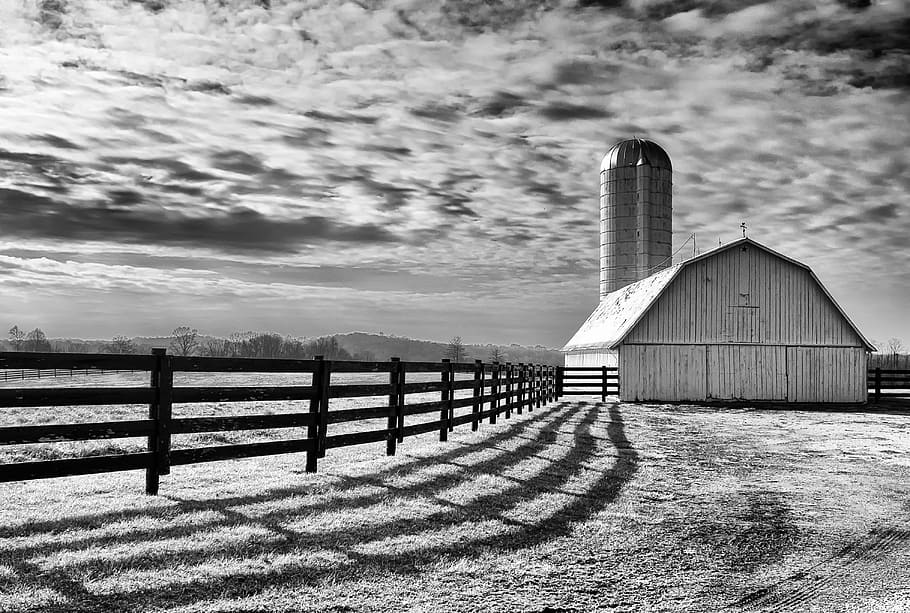
\includegraphics[width=0.9\textwidth]{example_image.png} % Replace with your results visualization.
\end{frame}

% Slide 10: Conclusion and Future Directions
\begin{frame}{More Results + Future Directions}

\end{frame}
\begin{frame}{References}

    \begin{itemize}
        \item Tipping, Michael E., and Christopher M. Bishop. \emph{"Mixtures of probabilistic principal component analyzers."} Neural Computation, 11.2 (1999): 443-482.
        
        \item Tipping, Michael E., and Christopher M. Bishop. \emph{"Probabilistic principal component analysis."} Journal of the Royal Statistical Society Series B: Statistical Methodology, 61.3 (1999): 611-622.
        
        \item Zhang, Zhihua, et al. \emph{"Probabilistic kernel principal component analysis."} Department of Computer Science, The Hong Kong University of Science and Technology, Technical Report (2004).
    \end{itemize}
    
    \end{frame}

    \begin{frame}
    
\textbf{M-Step:}
\begin{itemize}
    \item Update parameters for each mixture component:
    \begin{align*}
        \pi_i &= \frac{1}{N} \sum_{n=1}^N R_{ni}, \\
        \boldsymbol{\mu}_i &= \frac{\sum_{n=1}^N R_{ni} \mathbf{x}_n}{\sum_{n=1}^N R_{ni}}, \\
        \mathbf{W}_i &= \left(\sum_{n=1}^N R_{ni} (\mathbf{x}_n - \boldsymbol{\mu}_i) \mathbb{E}[\mathbf{z}_{n,i+1}]^T\right) \left(\sum_{n=1}^N R_{ni} \mathbb{E}[\mathbf{z}_{n,i+1} \mathbf{z}_{n,i+1}^T]\right)^{-1}, \\
        \sigma_i^2 &= \frac{1}{d} \sum_{n=1}^N R_{ni} \left[ \|\mathbf{x}_n - \boldsymbol{\mu}_i\|^2 - 2 \mathbb{E}[\mathbf{z}_{n,i+1}]^T \mathbf{W}_i^T (\mathbf{x}_n - \boldsymbol{\mu}_i) + \text{Tr}(\mathbf{W}_i^T \mathbf{W}_i \mathbb{E}[\mathbf{z}_{n,i+1} \mathbf{z}_{n,i+1}^T]) \right].
    \end{align*}
\end{itemize}
    \end{frame}


\end{document}
